\documentclass[a4paper, 14pt]{extarticle}

% Поля
%--------------------------------------
\usepackage{geometry}
\geometry{a4paper,tmargin=2cm,bmargin=2cm,lmargin=3cm,rmargin=1cm}
%--------------------------------------


%Russian-specific packages
%--------------------------------------
\usepackage[T2A]{fontenc}
\usepackage[utf8]{inputenc} 
\usepackage[english, main=russian]{babel}
%--------------------------------------

\usepackage{textcomp}

% Красная строка
%--------------------------------------
\usepackage{indentfirst}               
%--------------------------------------             


%Graphics
%--------------------------------------
\usepackage{graphicx}
\graphicspath{ {./images/} }
\usepackage{wrapfig}
%--------------------------------------

% Полуторный интервал
%--------------------------------------
\linespread{1.3}                    
%--------------------------------------

%Выравнивание и переносы
%--------------------------------------
% Избавляемся от переполнений
\sloppy
% Запрещаем разрыв страницы после первой строки абзаца
\clubpenalty=10000
% Запрещаем разрыв страницы после последней строки абзаца
\widowpenalty=10000
%--------------------------------------

%Списки
\usepackage{enumitem}

%Подписи
\usepackage{caption} 

%Гиперссылки
\usepackage{hyperref}

\hypersetup {
	unicode=true
}

%Рисунки
%--------------------------------------
\DeclareCaptionLabelSeparator*{emdash}{~--- }
\captionsetup[figure]{labelsep=emdash,font=onehalfspacing,position=bottom}
%--------------------------------------

\usepackage{tempora}

%Листинги
%--------------------------------------
\usepackage{listings}
\lstset{
  basicstyle=\ttfamily\footnotesize, 
  %basicstyle=\footnotesize\AnkaCoder,        % the size of the fonts that are used for the code
  breakatwhitespace=false,         % sets if automatic breaks shoulbd only happen at whitespace
  breaklines=true,                 % sets automatic line breaking
  captionpos=t,                    % sets the caption-position to bottom
  inputencoding=utf8,
  frame=single,                    % adds a frame around the code
  keepspaces=true,                 % keeps spaces in text, useful for keeping indentation of code (possibly needs columns=flexible)
  keywordstyle=\bf,       % keyword style
  numbers=left,                    % where to put the line-numbers; possible values are (none, left, right)
  numbersep=5pt,                   % how far the line-numbers are from the code
  xleftmargin=25pt,
  xrightmargin=25pt,
  showspaces=false,                % show spaces everywhere adding particular underscores; it overrides 'showstringspaces'
  showstringspaces=false,          % underline spaces within strings only
  showtabs=false,                  % show tabs within strings adding particular underscores
  stepnumber=1,                    % the step between two line-numbers. If it's 1, each line will be numbered
  tabsize=2,                       % sets default tabsize to 8 spaces
  title=\lstname                   % show the filename of files included with \lstinputlisting; also try caption instead of title
}
%--------------------------------------

%%% Математические пакеты %%%
%--------------------------------------
\usepackage{amsthm,amsfonts,amsmath,amssymb,amscd}  % Математические дополнения от AMS
\usepackage{mathtools}                              % Добавляет окружение multlined
\usepackage[perpage]{footmisc}
%--------------------------------------

%--------------------------------------
%			НАЧАЛО ДОКУМЕНТА
%--------------------------------------

\begin{document}

%--------------------------------------
%			ТИТУЛЬНЫЙ ЛИСТ
%--------------------------------------
\begin{titlepage}
\thispagestyle{empty}
\newpage


%Шапка титульного листа
%--------------------------------------
\vspace*{-60pt}
\hspace{-65pt}
\begin{minipage}{0.3\textwidth}
\hspace*{-20pt}\centering

\includegraphics[width=\textwidth]{emblem}
\end{minipage}
\begin{minipage}{0.67\textwidth}\small \textbf{
\vspace*{-0.7ex}
\hspace*{-6pt}\centerline{Министерство науки и высшего образования Российской Федерации}
\vspace*{-0.7ex}
\centerline{Федеральное государственное бюджетное образовательное учреждение }
\vspace*{-0.7ex}
\centerline{высшего образования}
\vspace*{-0.7ex}
\centerline{<<Московский государственный технический университет}
\vspace*{-0.7ex}
\centerline{имени Н.Э. Баумана}
\vspace*{-0.7ex}
\centerline{(национальный исследовательский университет)>>}
\vspace*{-0.7ex}
\centerline{(МГТУ им. Н.Э. Баумана)}}
\end{minipage}
%--------------------------------------

%Полосы
%--------------------------------------
\vspace{-25pt}
\hspace{-35pt}\rule{\textwidth}{2.3pt}

\vspace*{-20.3pt}
\hspace{-35pt}\rule{\textwidth}{0.4pt}
%--------------------------------------

\vspace{1.5ex}
\hspace{-35pt} \noindent \small ФАКУЛЬТЕТ\hspace{80pt} <<Информатика и системы управления>>

\vspace*{-16pt}
\hspace{47pt}\rule{0.83\textwidth}{0.4pt}

\vspace{0.5ex}
\hspace{-35pt} \noindent \small КАФЕДРА\hspace{50pt} <<Теоретическая информатика и компьютерные технологии>>

\vspace*{-16pt}
\hspace{30pt}\rule{0.866\textwidth}{0.4pt}
  
\vspace{11em}

\begin{center}
\Large {\bf Рубежный контроль № 1} \\
\large {\bf по курсу <<Разработка мобильных приложений>>} \\
\large <<Проверка усвоенного материала по теме форматирования контента виджетов и CustomPaint>>
\end{center}\normalsize

\vspace{8em}


\begin{flushright}
  {Студентка группы ИУ9-72Б Самохвалова П. С. \hspace*{15pt}\\
  \vspace{2ex}
  Преподаватель Посевин Д. П.\hspace*{15pt}}
\end{flushright}

\bigskip

\vfill
 

\begin{center}
\textsl{Москва 2023}
\end{center}
\end{titlepage}
%--------------------------------------
%		КОНЕЦ ТИТУЛЬНОГО ЛИСТА
%--------------------------------------

\renewcommand{\ttdefault}{pcr}

\setlength{\tabcolsep}{3pt}
\newpage
\setcounter{page}{2}

\section{Цель работы}\label{Sect::goal}

Реализовать мобильное приложение выполняющее построение простейших геометрических фигур.

\section{Задание}\label{Sect::task}

Приложение должно представлять из себя форму ввода входных данных и
виджет вывода результата. Приложение должно запускать на мобильном
устройстве.

Индивидуальный вариант:

Входные данные: координаты вершин треугольника в пространстве. Результат: вид проекции на плоскость xOy.

\section{Практическая реализация}\label{Sect::code}

Исходный код программы представлен в листинге~\ref{lst:code1}.

\begin{lstlisting}[language={},caption={Мобильное приложение выполняющее построение простейших геометрических фигур},label={lst:code1}]
import 'package:flutter/material.dart';
import 'dart:ui' as ui;

void main() {
  runApp(MyApp());
}

class Vertex {
  double x;
  double y;
  double z;

  Vertex(this.x, this.y, this.z);
}

class TriangleProjection extends StatefulWidget {
  @override
  _TriangleProjectionState createState() => _TriangleProjectionState();
}

class _TriangleProjectionState extends State<TriangleProjection> {
  final vertex1Controller = TextEditingController();
  final vertex2Controller = TextEditingController();
  final vertex3Controller = TextEditingController();
  List<Vertex> vertices = [];

  @override
  void initState() {
    super.initState();
    vertex1Controller.text = "0,0,0";
    vertex2Controller.text = "100,0,0";
    vertex3Controller.text = "0,100,0";
    _updateVertices();
  }

  void _updateVertices() {
    vertices.clear();
    vertices.add(_parseVertex(vertex1Controller.text));
    vertices.add(_parseVertex(vertex2Controller.text));
    vertices.add(_parseVertex(vertex3Controller.text));
    setState(() {});
  }

  Vertex _parseVertex(String vertexString) {
    List<String> values = vertexString.split(",");
    double x = double.parse(values[0]);
    double y = double.parse(values[1]);
    double z = double.parse(values[2]);
    return Vertex(x, y, z);
  }

  @override
  Widget build(BuildContext context) {
    return MaterialApp(
      home: Scaffold(
        appBar: AppBar(
          title: Text('Triangle Projection'),
        ),
        body: Padding(
          padding: EdgeInsets.all(16.0),
          child: Column(
            crossAxisAlignment: CrossAxisAlignment.start,
            children: <Widget>[
              TextField(
                decoration: InputDecoration(labelText: 'Vertex 1 (x,y,z)'),
                controller: vertex1Controller,
                onChanged: (_) => _updateVertices(),
              ),
              TextField(
                decoration: InputDecoration(labelText: 'Vertex 2 (x,y,z)'),
                controller: vertex2Controller,
                onChanged: (_) => _updateVertices(),
              ),
              TextField(
                decoration: InputDecoration(labelText: 'Vertex 3 (x,y,z)'),
                controller: vertex3Controller,
                onChanged: (_) => _updateVertices(),
              ),
              SizedBox(height: 16.0),
              Text(
                'Projected Triangle:',
                style: TextStyle(fontSize: 18.0, fontWeight: FontWeight.bold),
              ),
              SizedBox(height: 8.0),
              Container(
                width: 300,
                height: 300,
                child: CustomPaint(
                  painter: TrianglePainter(vertices),
                ),
              ),
            ],
          ),
        ),
      ),
    );
  }
}

class TrianglePainter extends CustomPainter {
  List<Vertex> vertices;

  TrianglePainter(this.vertices);

  @override
  void paint(Canvas canvas, Size size) {
    Paint paint = Paint()
      ..color = Colors.blue
      ..style = PaintingStyle.fill;

    Path path = Path();
    path.moveTo(vertices[0].x, vertices[0].y);
    path.lineTo(vertices[1].x, vertices[1].y);
    path.lineTo(vertices[2].x, vertices[2].y);
    path.close();

    canvas.drawPath(path, paint);
  }

  @override
  bool shouldRepaint(TrianglePainter oldDelegate) => true;
}

class MyApp extends StatelessWidget {
  @override
  Widget build(BuildContext context) {
    return MaterialApp(
      home: TriangleProjection(),
    );
  }
}
\end{lstlisting}

\section{Результаты}\label{Sect::res}

Результаты работы программы представлены на рисунках~\ref{fig:img1}~--~\ref{fig:img3}.

\begin{figure}[!htb]
	\centering
	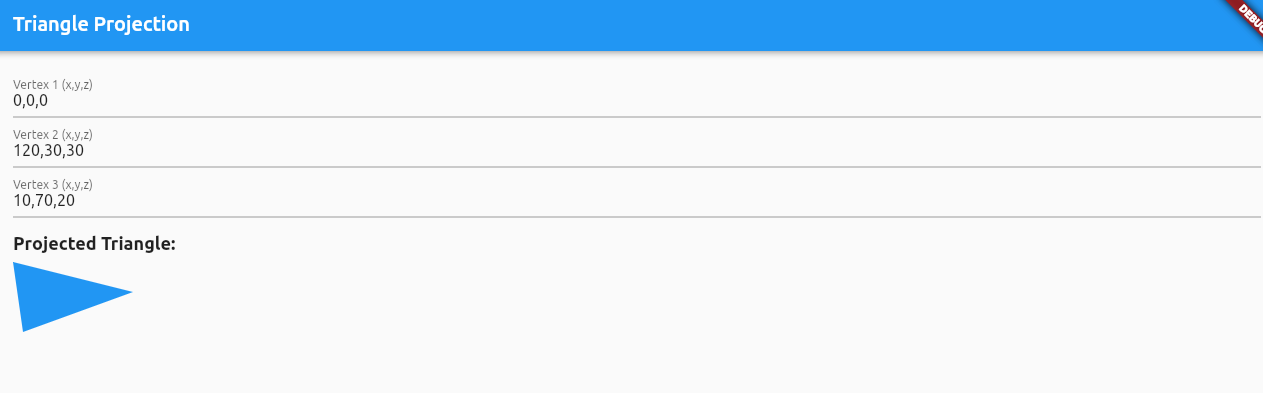
\includegraphics[width=0.8\textwidth]{img1}
\caption{Результаты}
\label{fig:img1}
\end{figure}

\begin{figure}[!htb]
	\centering
	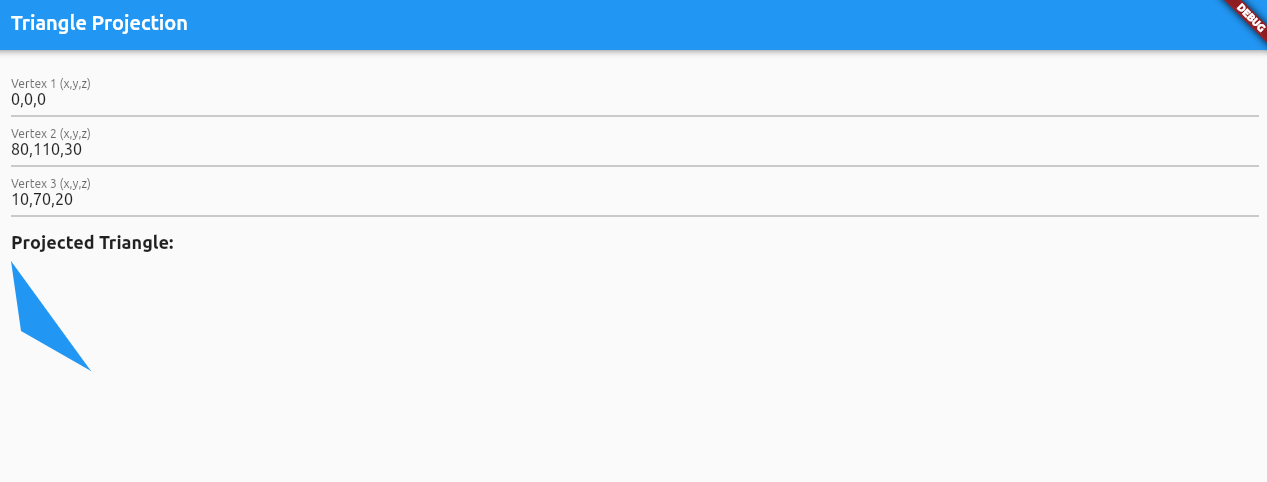
\includegraphics[width=0.8\textwidth]{img2}
\caption{Результаты}
\label{fig:img2}
\end{figure}

\begin{figure}[!htb]
	\centering
	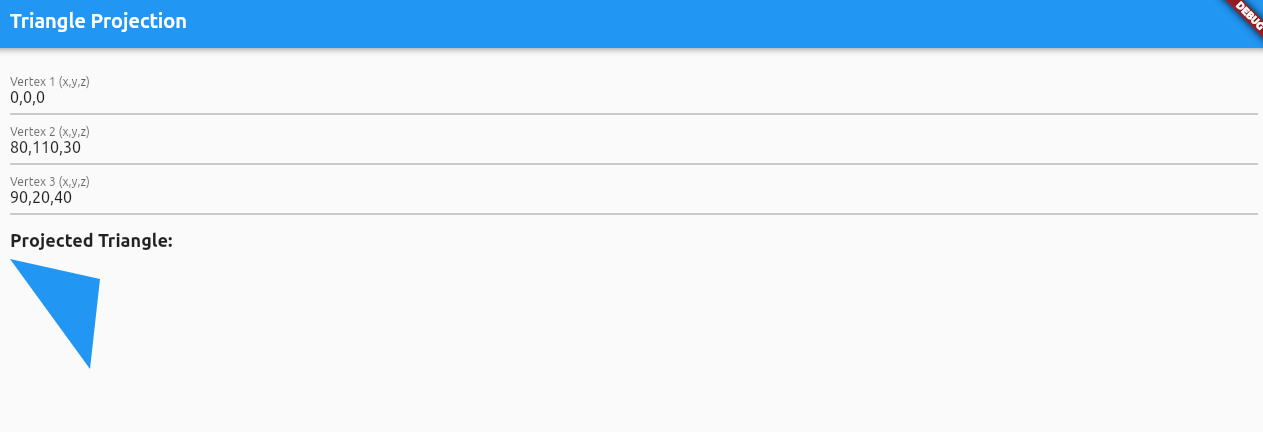
\includegraphics[width=0.8\textwidth]{img3}
\caption{Результаты}
\label{fig:img3}
\end{figure}

\section{Выводы}\label{Sect::conclusion}

В результате выполнения рубежного контроля было реализовано мобильное приложение выполняющее построение простейших геометрических фигур.

\end{document}
